\chapter{Analysis} \label{Analysis}

%Summary: describe how we get real numbers to put into previous part
%Goal: define and obtain real numbers from the previous part
\section{Benchmarks}
Discussion of benchmarks (show size vs resources) FFT, PFB,

\begin{figure}[ht!]
  \centering
    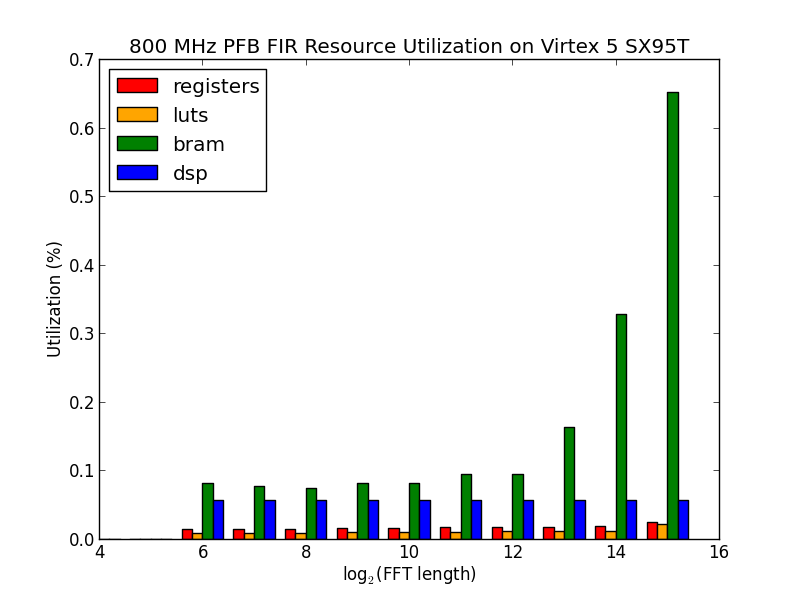
\includegraphics[width=0.49\textwidth]{Images/C6/pfb_bench.png}
  \caption{TODO}
  \label{fig: C6/pfb_bench.png}
\end{figure}

\begin{figure}[ht!]
  \centering
    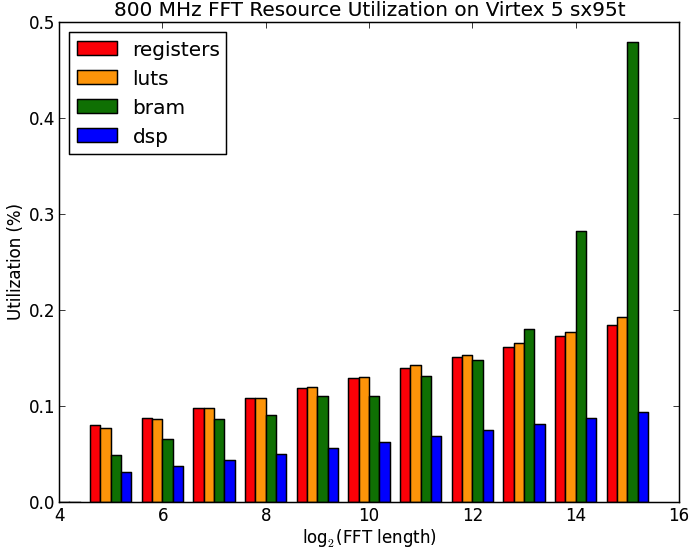
\includegraphics[width=0.49\textwidth]{Images/C6/fft_bench.png}
    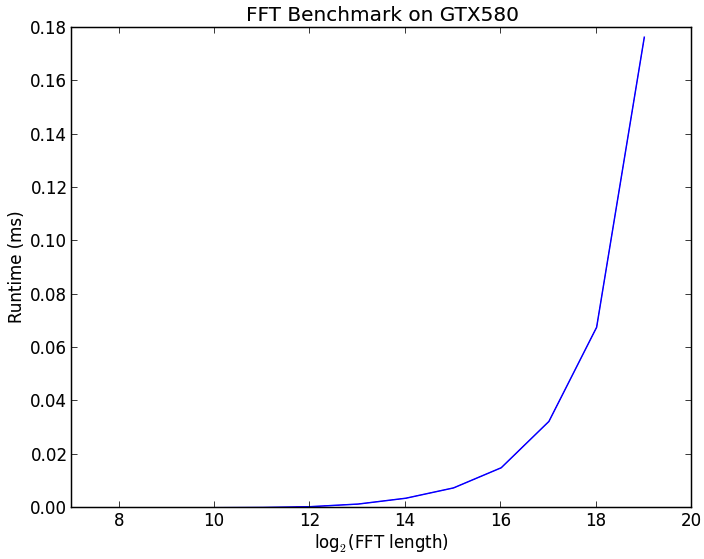
\includegraphics[width=0.49\textwidth]{Images/C6/fft_gpu_bench.png}
  \caption{TODO}
  \label{fig: C6/fft_bench.png}
\end{figure}

refer to casper fft model paper

refer to xgpu paper

\subsection{Cost}

\begin{table}
\begin{tabular}{| l | l | l | l | l | l |}
\hline  
\textbf{Platform} & Specification & Cost & Idle power & Average power & Maximum power \\
\hline  
ROACH & Virtex 5 SX95T & \$6,700 & 55 W & 65 W & 75 W \\
ROACH 2 & Virtex 6 SX475T & \$10,500 & 60 W & 70 W & 80 W \\
ROACH 3 & Virtex 7 VX980T & & 60 W & 70 W & 80 W \\
NRAO Server & GTX 580 & \$3,500 & 225 W & 400 W & 475 W \\
\hline  
\end{tabular}
\end{table} 

%TODO: Discuss this
Can also take into account donated hardware \\

\begin{table}
\begin{tabular}{| l | l | l | l | l |}
\hline  
GPU & Cost & Idle power & Average power & Maximum power \\
\hline  
GTX 580& \$500 & 125 W & 150 W & 175 W \\
GTX 680 & \$500 & & & \\
GTX 690& \$1,000 & & & \\
\hline  
\end{tabular}
\end{table} 



%Summary: case studies describing partitioning of realistic-scale instruments
%Goal: show successful application of tool to design of realistic instruments
%provide analysis comparing this to hand-designed instruments 
\section{Simple spectrometer}
Simple spectrometer placement

Include appropriate FFT or PFB benchmarks
\subsection{Cost}
\subsection{Power}

\section{Hi res spectrometer}
results for hi res spectrometer (gbt and seti)

Same benchmarks as before, just discuss large bw, multi stage fft
\subsection{Cost}
\subsection{Power}

\section{Pulsar processor}
extend to pulsar processor design

Need benchmarks for deconvolution algorithm (just cpu vs gpu? infeasible in fpga...) bug jonathon about this
\subsection{Cost}
\subsection{Power}

\section{Cross-correlator}
xgpu benchmarks, correlator placement

Need benchmarks for xengine
\begin{figure}[ht!]
  \centering
    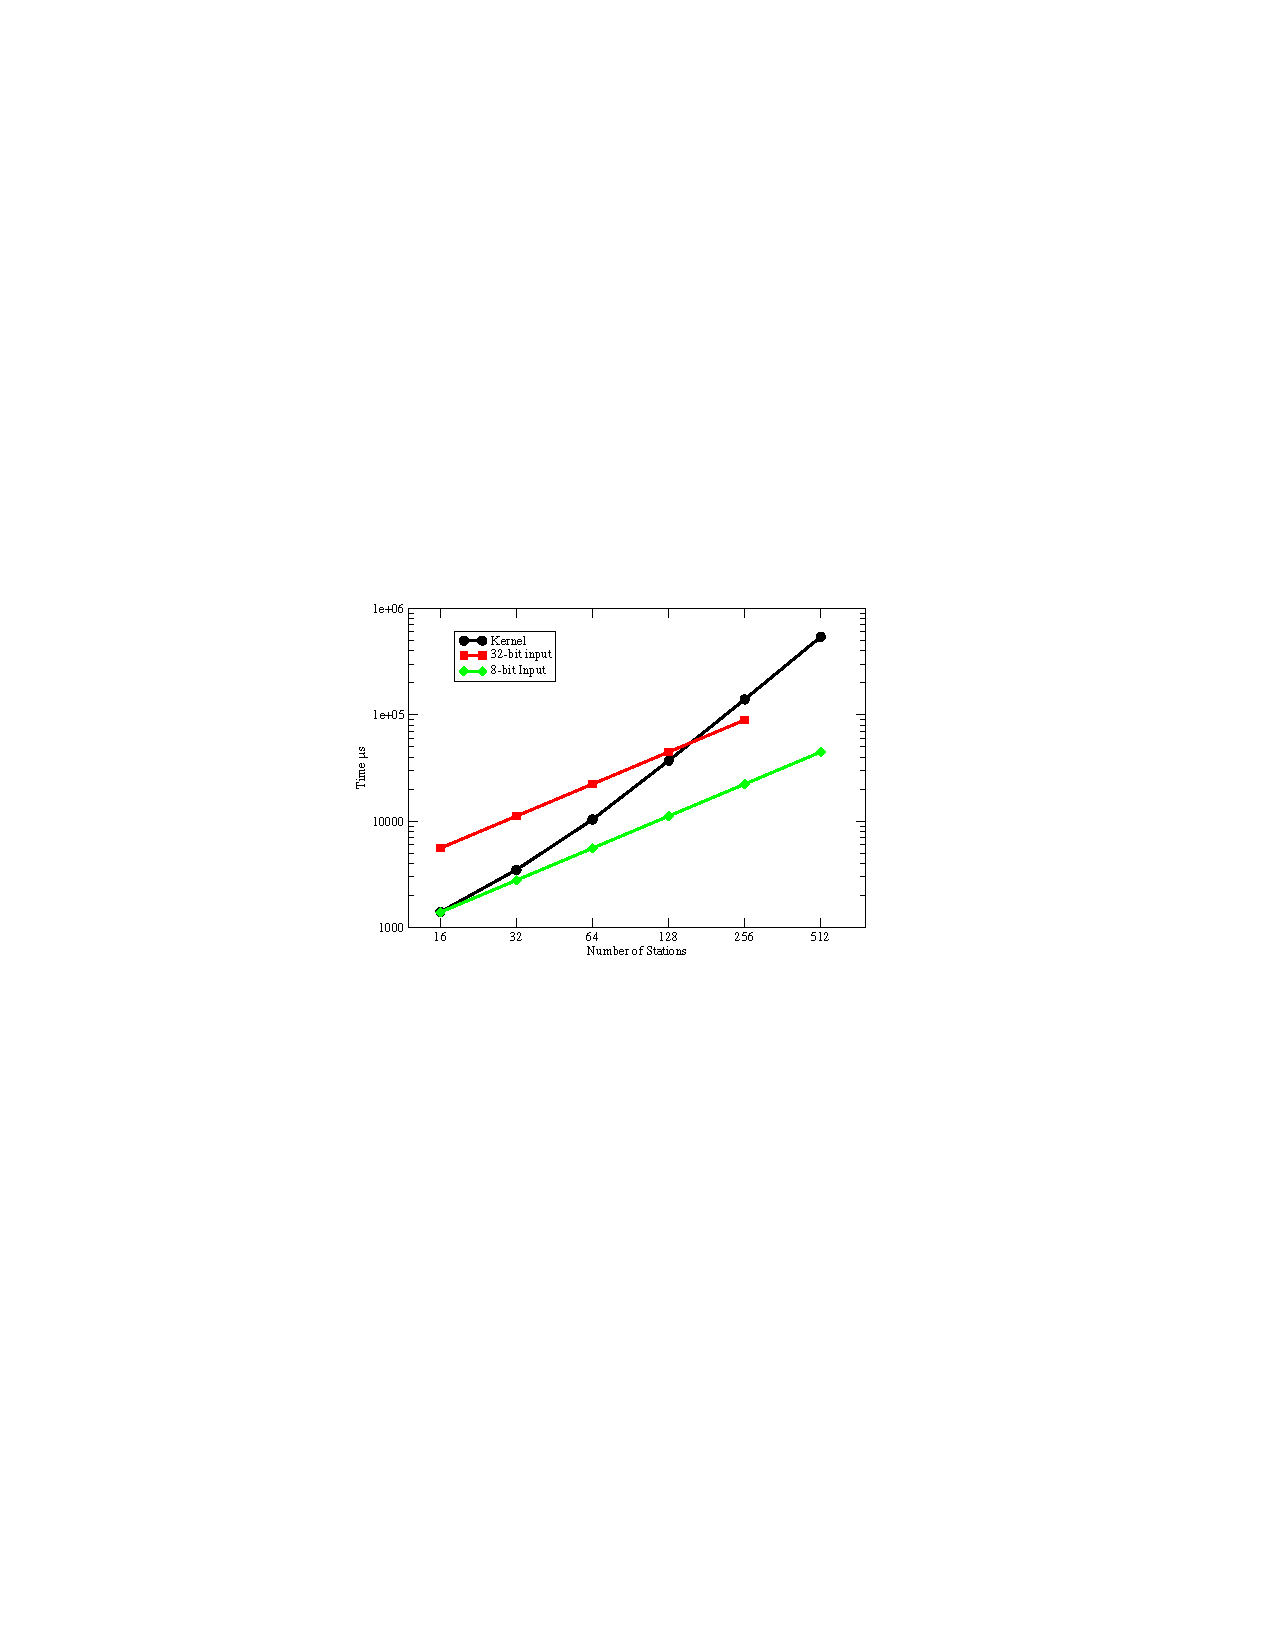
\includegraphics[width=\textwidth]{Images/C6/gpuxperformance.pdf}
  \caption{TODO}
  \label{fig: C6/gpuxperformance.pdf}
\end{figure}


\subsection{Cost}
\subsection{Power}
